\chapter{\ltwotau 分析道}\label{chap:1l2tau}
\ltwotau 聚焦于通过$ttH\rightarrow \tau^+\tau^-$衰变道寻找$t\bar{t}H$,其分析基本遵循文献~\cite{}的方法,
但是考虑到ATLAS对$\tau$ 的鉴别效率的提升,$\tau$ 的选择条件有相应的加强。
\ltwotau 的基本策略是经过初步的事例筛选之后,利用BDTG方法进一步区分信号与主要本底,即$t\bar{t}$(其中至少一个$\tau_{had}$是来源于$b$ 喷注,强子化衰变的$W$玻色子或者部分子簇射)。
最后$0<BDT\le 0.6$和$0.6<BDT\le 1.0$为信号比例较高的区域,$BDT<0.$为信号比例较低的区域,同时拟合三个区域得到信号强度。

\section{信号选择}
轻子,喷注以及$\tau_{had}$的筛选跟其他衰变道一致,轻子须通过\texttt{isolationFixedCutLoose},电荷误判压低变量和non-prompt轻子压低变量。所用的单轻子触发判选条件如下:
\begin{itemize}
\item 2015 data: $HLT\_mu20\_iloose\_L1MU15 || HLT\_mu50 || HLT\_e60\_lhmedium ||$ \\
$ HLT\_e24\_lhmedium\_L1EM20VH || HLT\_e120\_lhloose$;
\item 2016 and 2017 data: $HLT\_mu26\_ivarmedium || HLT\_mu50 || HLT\_e140\_lhloose\_nod0 ||$ \\
$HLT\_e26\_lhtight\_nod0\_ivarloose || HLT\_e60\_lhmedium\_nod0$.
\item The trigger lepton is required to have: pT$>27$ GeV/c in 2016 and 2017 data; pT$>21$ GeV/c for muon and 25 GeV/c for electron in 2015 data.
\end{itemize}
喷注\pt 要求至少25 GeV,$|\eta|<2.5$,以及\texttt{JVT}条件。\btag 是基于多变量学习方法的,所选的\btag 效率WP为70\%,\ltwotau 要求所有喷注都不是\btagged 的。
$\tau_{had}$须通过\texttt{tight} ID,\pt$>$25 GeV以及$|\eta|<2.5$筛选,其中$1.37<|\eta|<1.52$,即电磁量能器的空区,被排除掉。\\
\ltwotau 中的主要本底是$t\bar{t}$,为了压低此项本底,有两个办法:
\begin{enumerate}
  \item 因为至少一个$\tau_{had}$是来自$b$ 喷注,所以要求所选的$\tau_{had}$不是\btagged 的,可以去除25\%的假本底,而保持96\%的信号选择效率;
  \item 喷注数和$\tau_{had}$ \pt 可以帮助压低假本底,这是因为$t\bar{t}$倾向具有较少的喷注数和较低动量的$\tau_{had}$;但是它们作为BDTG的训练变量也许能够发挥更大作用,
    所以选择具有至少三个喷注和$\tau_{had}$ \pt 大于25 GeV的事例,与其他衰变道一致。
\end{enumerate}
信号的初步筛选可总结为:
\begin{itemize}
  \item 两个通过\texttt{tight} ID具有相反电荷的$\tau_{had}$,\pt$>$25 GeV,并且都没有\btagged;
  \item 两个$\tau_{had}$必须来自primary vertex;
  \item 一个匹配任一触发判选条件的孤立电子或$\mu$子;
  \item 至少三个喷注,其中至少一个是\btagged 的。
\end{itemize}
通过MC样本可以检查$\tau_{had}$的来源,定义来自希格斯玻色子或者矢量玻色子的为真(real)$\tau_{had}$,来自QCD喷注的为假(fake)$\tau_{had}$。图~\ref{Fig:1l2tau.truth}中两$\tau_{had}$分为fake-fake,fake-real,来自于$H\rightarrow \tau\tau$
的real-real,以及其他;可以发现$t \bar t H$ 的纯度非常高,达到90\%,而主要来源于$t\bar{t}$的本底至少有一个fake。
图~\ref{Fig:1l2tau.truth}也给出假$\tau_{had}$的来源分布,大部分来源胶子喷注。由图中还可以发现相反电荷与相同电荷具有非常相似的分布,
其稍微的不同会考虑成假本底的形状误差,通过比较相同电荷与相反电荷的$t\bar{t}$样本得到,这会在章节~\ref{sec:1l2tau_sys}中讨论。
\begin{figure}[htbp]
\centering
\begin{center}
  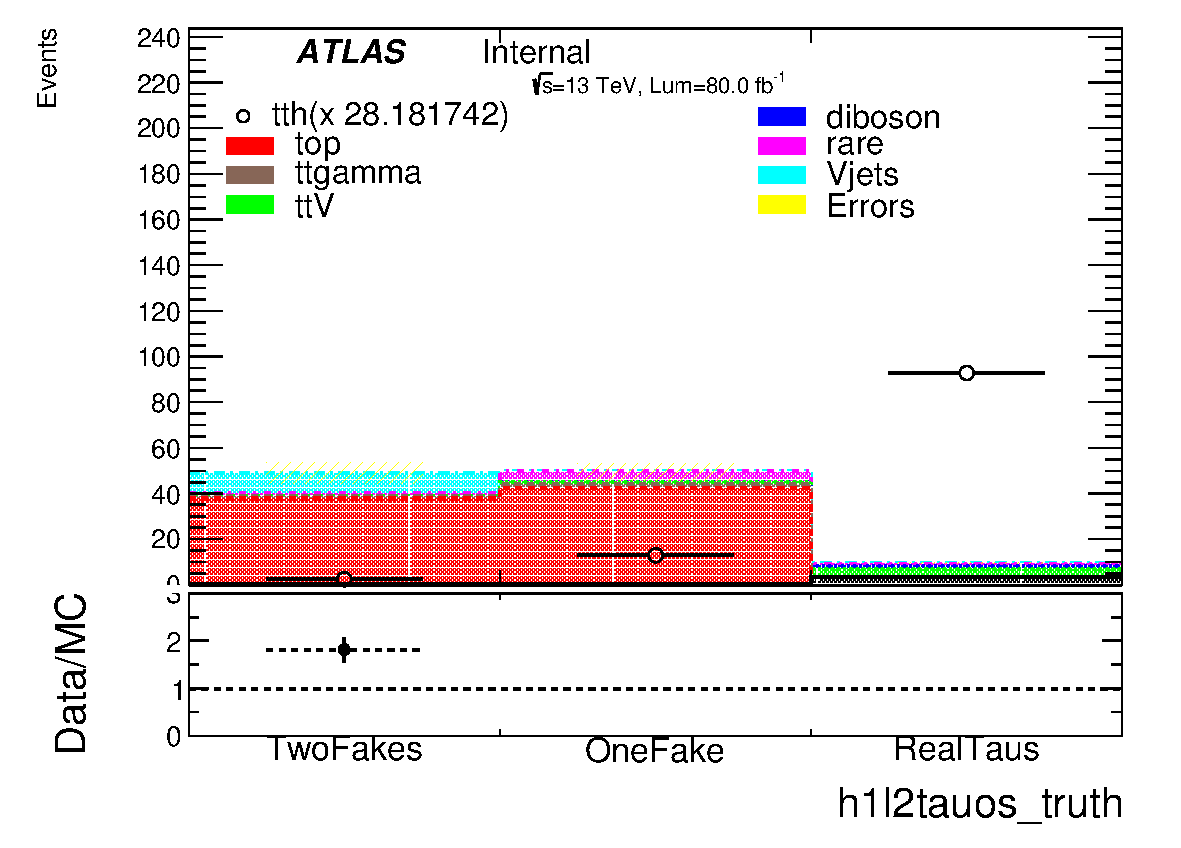
\includegraphics[width=0.45\textwidth, keepaspectratio]{fig/OneLepTwoTaus/Plots_h1l2tauos_truth_signal.pdf}
  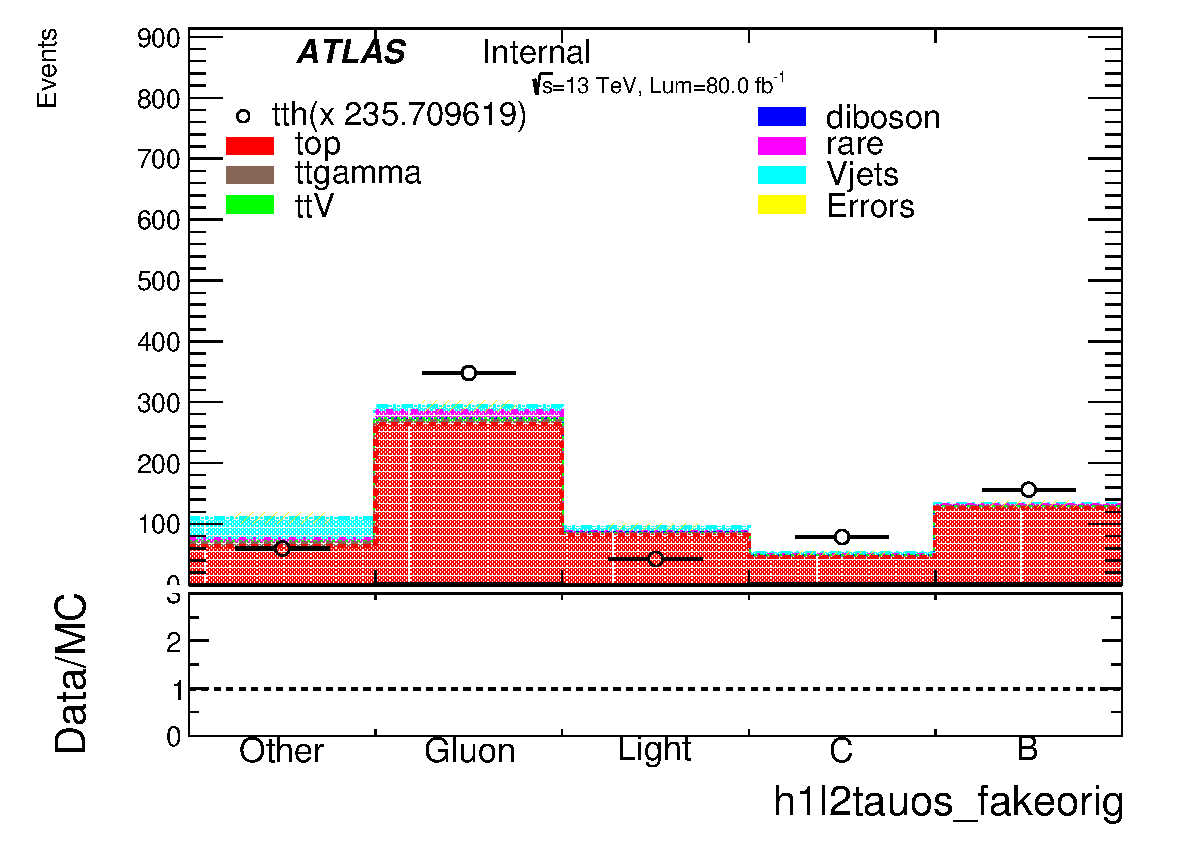
\includegraphics[width=0.45\textwidth, keepaspectratio]{fig/OneLepTwoTaus/Plots_h1l2tauos_fakeorig_signal.pdf}
  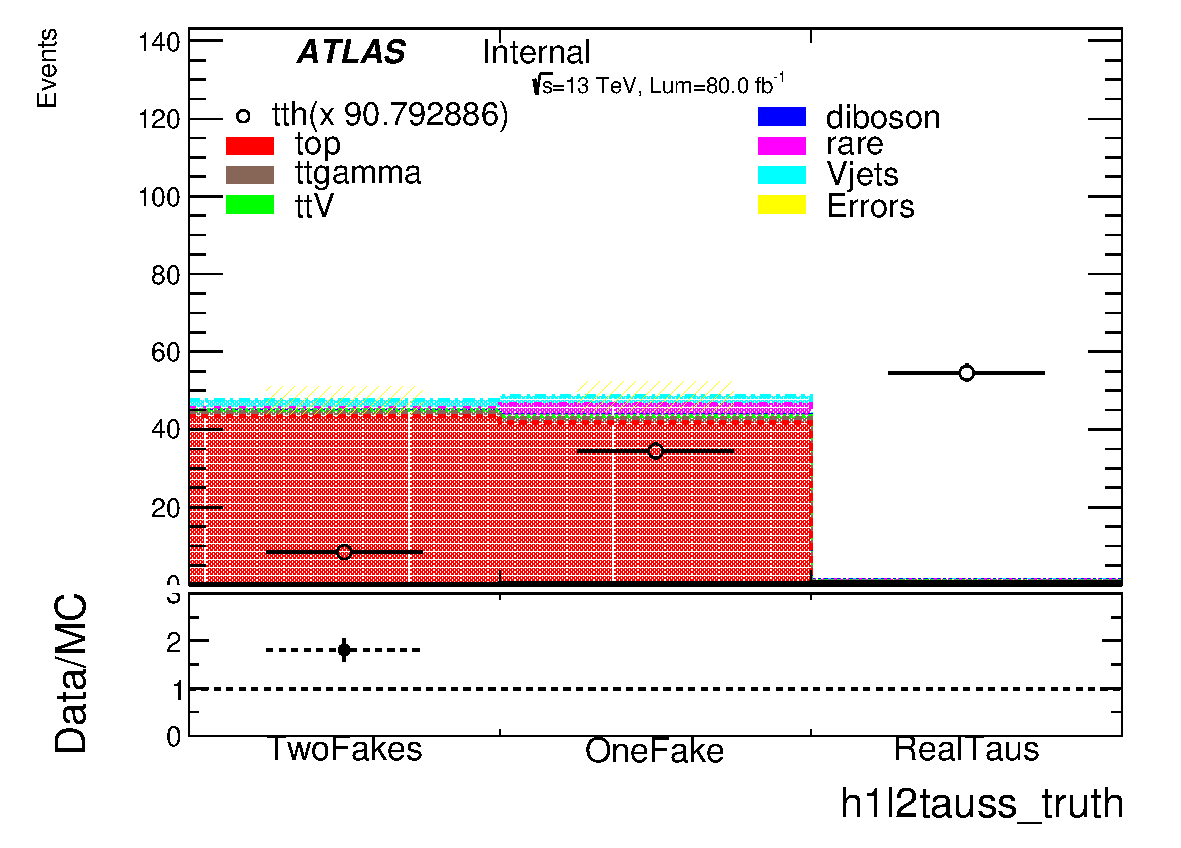
\includegraphics[width=0.45\textwidth, keepaspectratio]{fig/OneLepTwoTaus/Plots_h1l2tauss_truth_signal.pdf}
  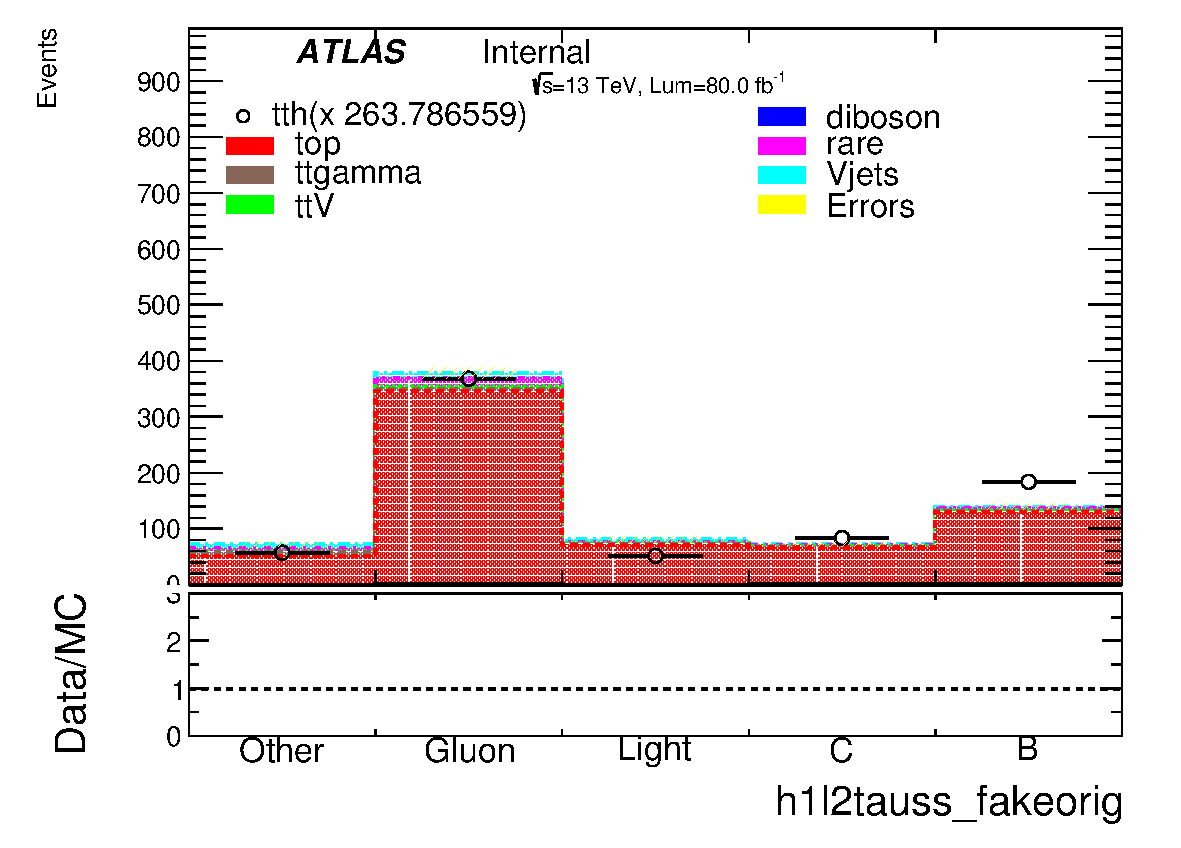
\includegraphics[width=0.45\textwidth, keepaspectratio]{fig/OneLepTwoTaus/Plots_h1l2tauss_fakeorig_signal.pdf}
\end{center}
\caption{The original di-tau events are classified based on the Monte Carlo truth as fake-fake, fake-real, real-real from Higgs decay or 
anything else, respectively, in left and the origin of the fake taus are shown in right. The top row for OS and the bottom row for SS. The signal is normalized to the total background in each plot.}
\label{Fig:1l2tau.truth}
\end{figure}

\section{Fake本底估计}

\section{MVA研究}

\section{系统误差}\label{sec:1l2tau_sys}
